\chapter{Sources}

\label{ch:sources}

The chapter on sources is devoted to the description of the theory, used for the thesis realisation, overview of the existing solutions of similar problems and introduction of the used technologies.

\section{Agile software development}

The aim of the web application is to introduce and teach how to use the selected methodologies of agile programming. They are based on principles of Agile software development, stated by authors of Manifesto for Agile Software Development \cite{manifesto}.

This approach advocates adaptive planning, evolutionary development, empirical knowledge, and continual improvement, and it encourages rapid and flexible response to change \cite{swdev}. Detailed planning of a large amount of the software process at once for a long span of time is a fragile approach and leads to further growing number of problems, when there is a need of change. The larger the is the system, the more difficult it may be to add new features, and the more difficult is it to fix bugs, and the more resources it requires. The agile methods are rather adaptive than predictive. So they welcome change, they are able to adapt and even thrive on change \cite[From Nothing, to Monumental, to Agile]{agile_fowler}. 

Agile approach provides this by iterative development, which means a frequent production of working versions of the final system that have a subset of the required features. These working systems are short on functionality, but should otherwise be faithful to the demands of the final system. They should be fully integrated and as carefully tested as a final delivery. The other feature is a feedback mechanism to estimate the situation \cite[Controlling an Unpredictable Process - Iterations]{agile_fowler}. 

The overview on the methods, on how may they affect the process of software development and how are they represented in the project are covered in the following sections.

\subsection{Extreme programming}

One of the most efficient, time-proven and used frameworks of Agile software development is Extreme programming, also knows as XP. It has already been proven to be very successful at many companies of all different sizes and industries world wide \cite{xp_intro}.

One of the authors of Manifesto for Agile Software Development American software engineer Kent Beck is a contributor to XP \cite{xp_explained}. This method focuses on the practical rather than management aspects of the development. The aim of the XP methodology is to improve software quality and responsiveness to changing customer requirements.

The name ``Extreme'' is taken from the idea that the beneficial elements of traditional software development are taken to ``extreme'' levels \cite[Preface]{xp_explained}.

As soon as XP is a framework of Agile web development, it includes iterations and feedbacks. The planning and feedback loops are illustrated on the image \ref{fig:xp_loop}. This approach assumes three levels of plans, the first one for the next a few months, the second one for the next iteration and the last one for the next task within an iteration. The plans are expected to be constantly recreated during the whole development process. Unit testing and acceptance coverage is a very important part of every stage of an XP project. XP provides feedback throughout the whole project on many levels and in many ways \cite[Planning/Feedback loops]{xp_intro}.

Also, while planning, new functionality can be added only when it is necessarily required. Otherwise, most of the unnecessary changed would be removed later, slow down the process and need excessive resources. The design should be simple, so the program would be ready for unexpected changes \cite{xp_early}.

\begin{figure}[h]
    \centerline{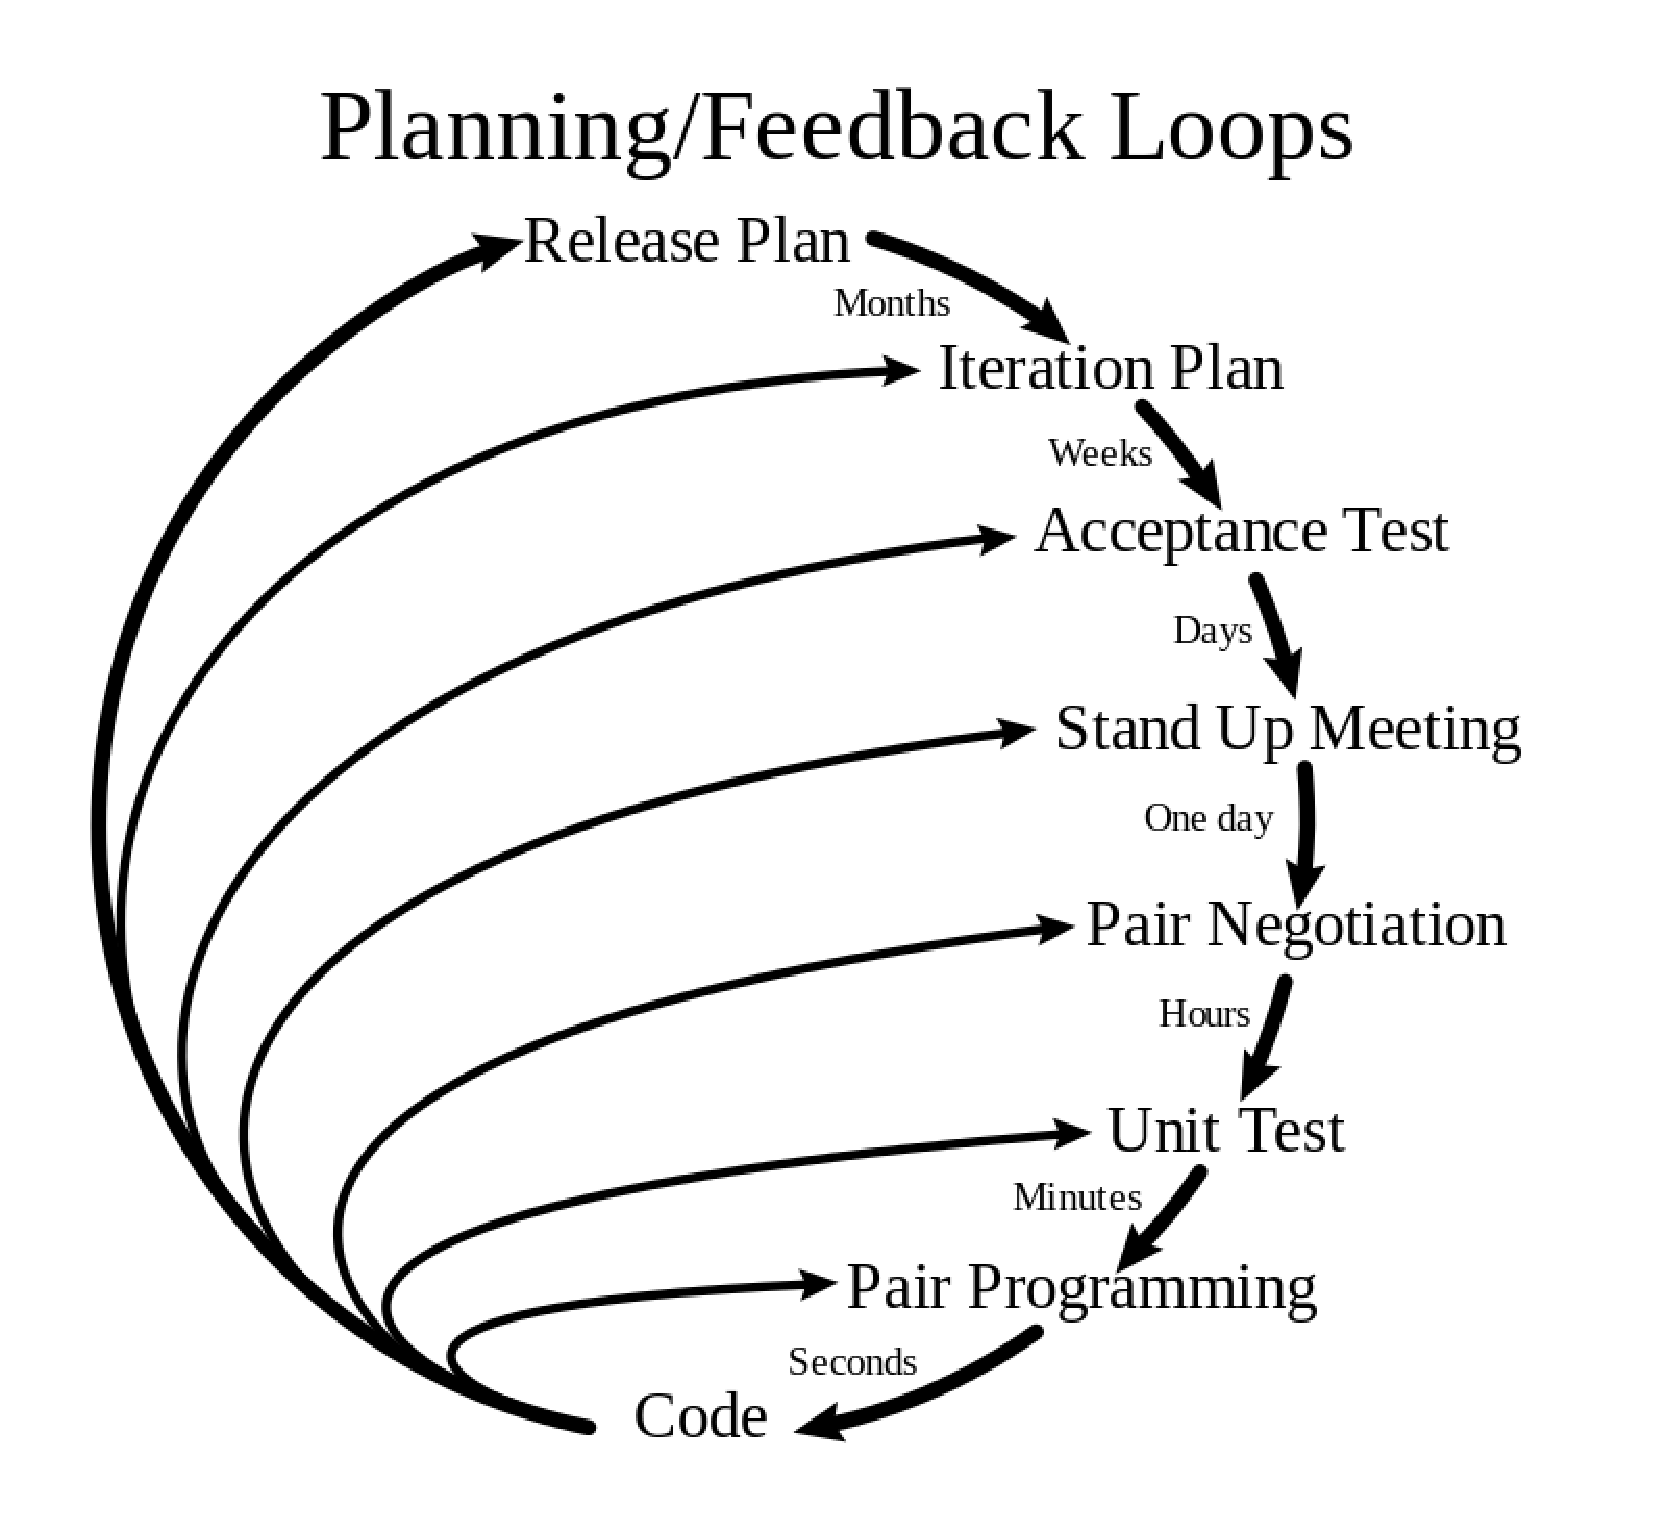
\includegraphics[width=0.6\textwidth]{images/xp_loop}}
    \caption{Planning and feedback loops in extreme programming}
    \label{fig:xp_loop}
\end{figure}

The web application, which would be the result of the work on the bachelor thesis, is designed to encourage the creation of the projects to solve in such a way, so students would develop a program in iterations and would receive a feedback. Each iteration would have exercises, which would lead through the work on the project. A sample project is an example of such a tasks, the exercises a grouped into three iterations. It covers the process of development an adaptive to changes program out of a fragile one, while learning the main XP methods. The sample project is described in detail in Chapter \ref{ch:sample_course}.

\subsection{Methods of XP}

XP is built on the best practices, they are combined in a way that they complement and control each other \cite[Foreword]{xp_explained}. The methods of XP, which were or may be used in the web application, will be introduced in the following subsections.

\subsubsection{Test-Driven Development (TDD)}

The technique of Test-Driven Development, also known as TDD, was developed by already mentioned Kent Beck, one of the authors of Manifesto for Agile Software Development \cite{tdd_example}.

This practice supports work in short development cycles. It includes writing of the test cases, which cover the requirements, and only after the implementation is made to pass these tests. Also good written tests provide continuous feedback for the programmer, which is also essential for Agile development \cite{tdd_dp}. There are different techniques to work with legacy code efficiently, mainly for making modifying it, but TDD is the common feature \cite[Test-Driven Development (TDD)]{lc_effectively}.

The key feature of the web application is that it would force using TDD to solve the tasks. A student would program within the provided IDE with editors for the source code and for the tests to be run on it. These tests would be run within the web application and a student would get a feedback. The range of the details provided with test result would be determined by the exercise author. 

The sample project shows how work with legacy code can be improved with use of TDD techniques. The first iteration provides exercises on debugging the legacy program. The aim is to find bugs in the legacy program and fix them, but keep the original structure of the code. The user should write his/her own tests to find the bugs and fix them. The second iteration is aimed to add some features to the code, bud to keep the original structure of the code as well. Tests, used in a previous iteration, with the new tests would be needed to accomplish the iteration requirements. The last iteration is made up with numerous exercises on refactoring. The TDD techniques are essential to proof that the program would remain correct.

\subsubsection{Refactoring}

Code refactoring is the process when a software system is changed in such a way that it does not alter the external behaviour of the code, thus improves its internal structure. The idea of factoring is different from general code cleanup, because it is less risky and invasive. Series of small structural modifications take place. Moreover, the tests provide a confidence that code remains correct \cite{lc_effectively}. As a result, the code is cleaned up and the chances of introducing bugs reduce. Refactoring is about improving the code, which has already been written. It is important to create a good design firstly and then to code. But refactoring is the opposite of this practice, because it deals with bad, chaotic design to rework it into a good one \cite[Preface]{ref_ec}.

Refactoring is a common part of an efficient work with legacy code, when there is a need in the design improvement. Such a software change would make its structure more maintainable, while the behaviour would be kept \cite{lc_effectively}.

Also there are cases, when refactoring is not recommended yet. For example, when there is a need to rewrite the whole code from the beginning instead. It may happen, when the code works mostly incorrectly. It is also recommended to avoid refactoring, when the deadline is close, because refactoring may remain unfinished. It would lead to a raise in cost of maintenance as well as an code, which was not reafactored at all \cite[Preface]{ref_debt}.

The web application also would make practice with refactoring possible. Refatoring a legacy code exercise are introduced in the sample project. Since refactoring should not be made when there are many mistakes in the code, the refactoring exercises take place in the third, last iteration. At this moment, after the previous two iterations are completed successfully and passed all the tests, the code would be correct. Each of the numerous exercises is about a single step of the code change, exercise description and title would reference to the book "Clean Code" by Robert C. Martin \cite{clean_code}. It is one of the mostly recommended books for software development, and for a good reason. During and after refactoring the code should maintain correct, and it can be provided by tests, written by the user.

\subsubsection{Mature optimisation}

Optimisation is similar to refactoring, they both keep the functionality of the code. Although they have different goals. Refactoring changes the program structure, so it is easier to maintain. Optimisation makes changes in the resources, used by the program, e.g. time or memory \cite{lc_effectively}. Refactoring makes code readable and understandable, while optimisation of the code to achieve the needed performance often makes code harder to understand \cite{ref_ec}.

Optimisation may not always be performed optimally and save the resources as a result. Donald Knuth, an American computer scientist and professor at Standford University, mentioned this issue in his paper "Structured Programming With go to Statements" \cite{knuth_goto}. He wrote that the programmers waste too much time on worrying about the speed of not crucial software parts, what makes negative impact, when maintenance and debugging are considered. So he concludes, that premature optimisation is the root if the all evil. As soon as optimisation may reduce readability and make the system more complex, it may be harder to maintain and debug it. Because of that, it is realised at the end of the development. This practice is sound with Agile development and XP principle of development of only the necessary parts only when they are needed.

The web application also enables an illustration of this point to a student. The sample project contains an exercise on refactoring, where it is required to change the way of computing the result. Such a task is within the last steps of the refactoring process. The steps after make no influence on the structure.

\subsubsection{Pair programming}

Pair programming is a technique, when the code for a single task is written by two people. The first programmer, the driver, has control of the computer and actively implements the program, and the other, the observer, provides feedback with reviewing the written code and thinks strategically about the work direction \cite{pair_prog}. Feedback is also provided during pair programming. 

Web application would allow to work on assignments in pairs.

\subsubsection{User story}

User story is a customer's functional requirement.

Ron Jeffries, one of the authors of the Manifesto for Agile Software Development \cite{manifesto}, proposed a ``Three Cs'' formula for user story creation. The first ``C'' is for Card, on which user stories are written. It does not contain all the information that makes it up, but it has the needed information to identify it. There may be notes of cost and priority of the requirement. The second ``C'' is for the Conversation between the stakeholders, which particularly takes place during the planning. The third one is for the Confirmation, which is provided by an acceptance test, telling is the aims of the conversation have been reached \cite{rj_3c}.

In XP it may be used as an instrument for stating the requirements and providing a feedback, also the tests may be based on user stories. In the web application the user stories would be used to formulate the requirements needed to fulfil to accomplish an exercise.

\subsection{Practical use of XP}

According to the 12$^{th}$ annual State of Agile survey, which was taken in 2018, only 1\% of respondents' organisations use XP \cite{agile_survey}. Another Agile framework, Scrum, is used by the majority of 56\%. However, hybrid of another Agile framework, Scrum, and XP, is used by 6\% of companies. This hybrid, known as ScrumXP, combines practices of Scrum project management and programming practices of XP.

Extreme programming is not that popular practice because of several reasons. The following reasons are the ones which are associated with the mentioned techniques.

It may seem irrational, even impossible to write tests before the code exists, which is the idea of Test-Driven Development. Even writing tests in general is not a common practice. As mentioned previously in a corresponding subsection, the benefits are real.

As about pair programming, it is counter intuitive as well. But as a result, the software quality may be increased within a lesser time than if two programmers worked separately. On one hand, programmer working by himself gets distracted more often, pair programming simplifies testing, getting feedback and code review, programmers feel more confidence in their. But on the other hand, it cannot work for every programmer or company. Most of the developers, especially the experts, prefer working on their own \cite[Two by Two]{xp_howto}.

The aim of the web application is to explain such an approach, show examples of use and to teach how to get benefits from it.


\section{Existing solutions}

The web application would be presented in a form of an interactive online course. Its interface and control would be inspired by the existing platforms, introduced in the following subsections.

\subsection{Similar Bachelor and Master theses result works}

Results of work on Bachelor and Master theses at Comenius University in Bratislava, faculty of Mathematics, Physics and Informatics will be introduced in the following subsections.

\subsubsection{Web learning programming using TDD technology}

This Bachelor thesis (original title: Webová výuka programovania pomocou metodológie TDD) was written by Tomáš Bočinec in 2018.

The resulting web application is a good example of a simple and functional learning environment. The web application for learning Agile programming methods would use similar mechanism to compile the provided source code and tests, to run the tests and return the result. But more modern and efficient technologies would be used. And the exercises would have more specific structure for practising the Agile programming methods. The details are introduced in the next section \ref{sect:tech} on used technologies.

% Other similar environments, which are the results of Bachelor and Master theses

% \subsubsection{Web environment for development in C++}

% This Master thesis (original title: Webové vývojové prostredie pre jazyk C++) was written by Daniel Krajč in 2010. The web application was a result of the work on it. This web application was used at the faculty for subject Programovacie techniky v C++ for teaching programming in a corresponding programming language \cite{mt_krajc}.


% \subsubsection{Web learning programming in C++ using Unit testing}

% This Bachelor thesis (original title: Webová výuka programovania v C++ pomocou jednotkového testovania) was written by Viliam Vakerman.

% \subsubsection{Web environment for learning code refactoring}

% This Bachelor thesis (original title: Vývojové prostredie pre učenie sa refaktorizácie kódu) was written by Ivan Latták.


\subsection{Similar web applications}

\subsubsection{Codecademy}

Codecademy is an education company, which positions itself as an alternative to classical education. Web application they provide is a result of rethinking current approach on education \cite[About]{codecademy}.

There are courses of Web Development, Programming and Data Science. In fact the exercises focus on programming languages syntax, the knowledge of which depends mostly on practising. Basic principles behind it, important for the beginners as well, are left without the attention. These principles are mentioned and learned a lot at universities, which are criticised by Codecademy. However, the courses are great for the ones, whose aim is to gain knowledge of a programming language itself without any learning material above.

Codecademy popularises Test-Driven Development, and offers a course on it for an enrolment payment. Also the web offers code reviewing and receiving a feedback, but Codecademy does not provide this functionality directly and the other service Git Hub is used for it.

The web application for learning Agile programming methods would introduce the idea behind the techniques used in exercises, otherwise they would remain to seem counter intuitive and not understood.

Codecademy web page and development environment are very user-friendly and pleasing to the eye. The interface of the web application for learning Agile programming methods would be designed to produce the same impression. It is shown on the screenshot: \ref{fig:codecademy}. The environment is divided into three panes. The left contains the exercise content, the middle one is an editor, and the right one shows an output in the built-in web browser.

\begin{figure}[h]
    \centerline{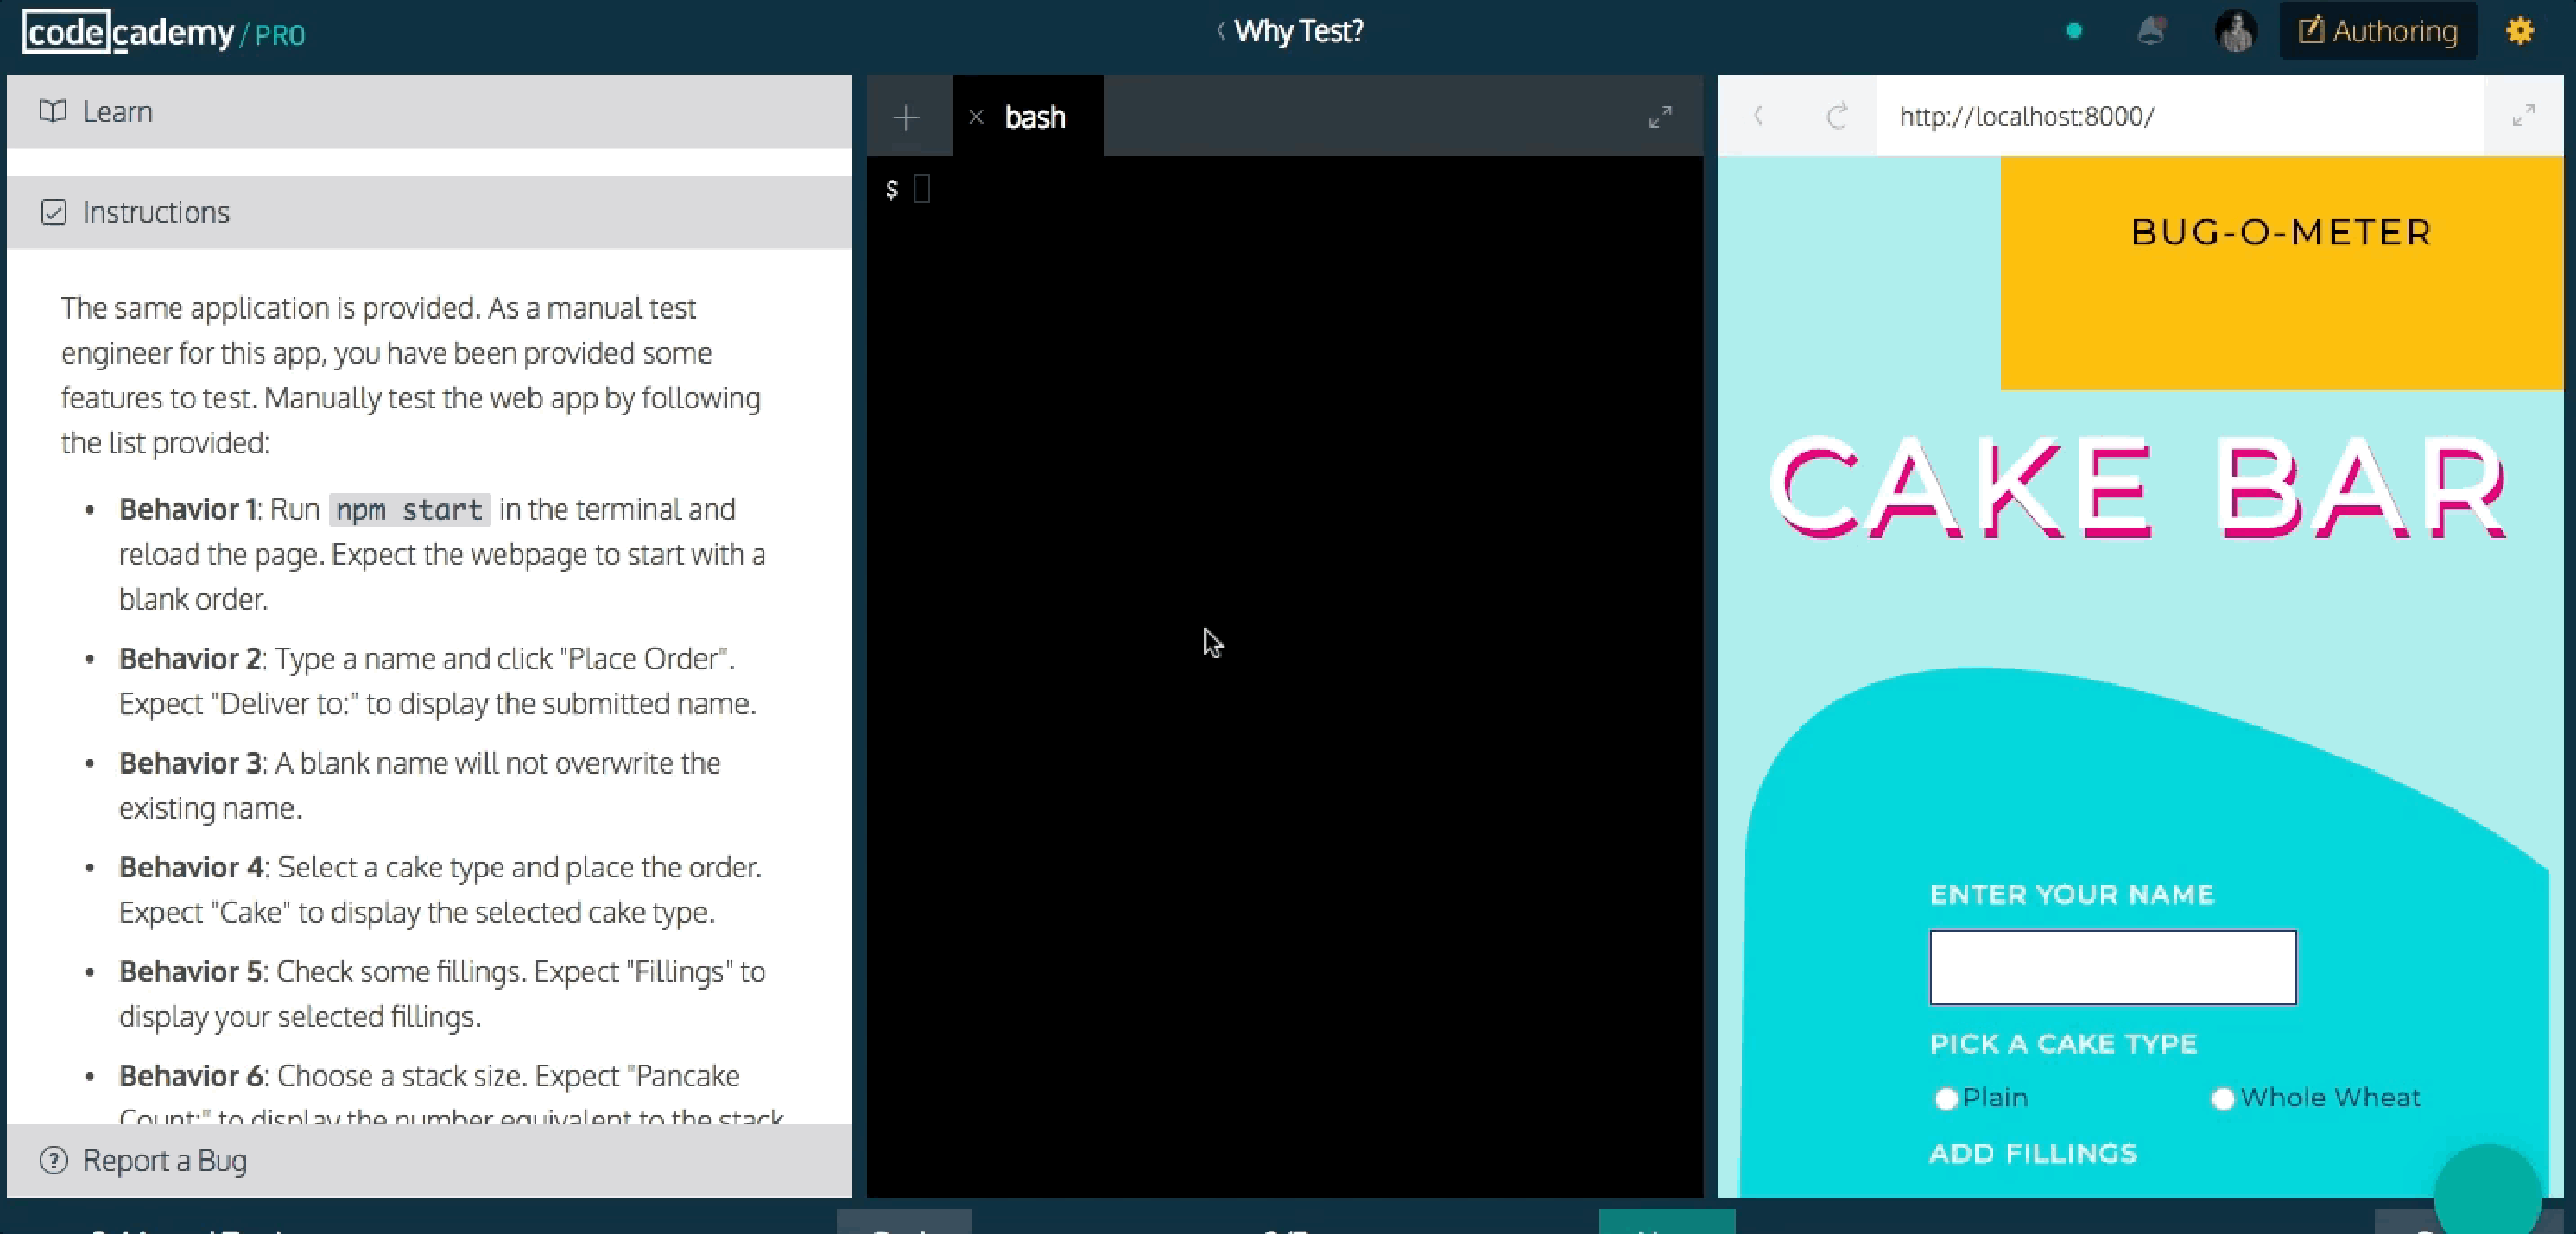
\includegraphics[width=0.9\textwidth]{images/codecademy}}
    \caption{Development environment at Codecademy}
    \label{fig:codecademy}
\end{figure}

\subsection{freeCodeCamp}

Another online courses interactive platform is freeCodeCamp. Moreover, it is a community, which helps to learn programming for free and to get experience by contributing to open source projects used by nonprofit organisations. They offer practising with completing coding challenges and work on the projects. Also joining the study group in the students' city to code in-person is encouraged. On the opposite to Codecademy, freeCodeCamp does not position itself as a high education alternative. They encourage to study to earn a degree and to pursue the courses they provide \cite{feecodecamp}.

Some of the courses take form of projects, this approach would be used in the web application for learning Agile programming methods. The reason is that it depicts the principles and enables practising in the best way. 

Like in Codecademy, the web does not provide a functionality of code review of the projects directly. The other service Git Hub is used for it. They introduce a term User Story while working at the projects to introduce the project requirements. In the web application for learning Agile programming methods the user stories would be used to formulate the requirements needed to fulfil to accomplish an exercise.

\section{Technologies to be used}
\label{sect:tech}

The technologies, which would be used in the web application for learning Agile programming methods, are introduced and analysed in the following subsections. These technologies are used in the web application prototype.

Web application would use client-server architecture. The server part would provide the central functionality. The clients would connect to it and request performing the tasks, and the server would provide the results.

\subsection{Client side}

The client side application would use Angular. It a structural framework for dynamic web applications, which is based on JavaScript pment to initialize, develop, scaffold, and maintain the application, add new components, modules and services \cite{angular_cli}. Angular enables development of modular and reusable dynamical web applications.

\subsubsection{TypeScript}
The Angular framework is built entirely in TypeScript, and it is used as a primary 
language. As soon as browsers cannot execute TypeScript directly, the code must be converted into JavaScript with tsc compiler \cite[TypeScript Configuration]{angular}.

\subsubsection{HttpClient}

The front-end of the application communicates with backend services over the HTTP protocol. The web browsers support APIs for making HTTP requests of two different types: the XMLHttpRequest interface and the fetch() API. Angular offers the HttpClient, which is a simplifies HTTP API that rests on the XMLHTTPRequest interface exposed by browsers. Also it includes testability features, typed request and response objects, request and response interception, Observable APIs, and streamlined error handling \cite[HttpClient]{angular}. Angular makes use of observables as an interface to handle a variety of common asynchronous operations. The observables provide support for passing messages between publishers and subscribers \cite[Observables \& RxJS]{angular}. 

\subsubsection{Sass}

User interface would be implemented using HTML5 and CSS3. Sass, a preprocessor scripting language, would be compiled into CSS. The CSS preproccessors are responsible for recompiling the existing code into the format compliant to the CSS standard. Sass provides such a functionality as multilevel nesting, what improves readability of the code and reduces its volume. It also allows to declare variables. CSS3 also has such a feature, but it is not supported by all the browsers, i.e. Internet Explorer. Mixin insertion solves the problem of a need to duplicate the code. Also Sass enables expanding, inheriting and importing the styles \cite{sass}.

\subsection{Server side}

The server side Java application would use Spring Framework 5.0. The core functionality of the web application is compilation of the source code and tests, running these tests and returning the result. When the server part would get a request to provide this functionality, the code would be compiled.

\subsubsection{Maven}

Maven is a software project management and comprehension tool. Based on the concept of a project object model (POM), Maven can manage a project's build, reporting and documentation from a central piece of information. Maven automates such a tasks as downloading dependencies, putting additional jar files on a project classpath, compiling source code, running tests, packaging compiled code into deployable artifacts such as JAR, WAR and ZIP files, and deploying these artifacts to an application server \cite{maven}. Such an automatising assures avoiding the mistakes, which may occur when building the software manually.

\subsubsection{Spring}

The Spring Framework is an open source developed by Pivotal Software application framework and inversion of control container for the Java platform. It provides comprehensive infrastructure support for developing Java applications. 

It contains modules, which make development faster and simpler. Spring Boot is an extension of the Spring Framework, a convention-over-configuration solution. In other words, it makes it easy to create applications, which can ``just run'' \cite{spring_boot}.

\subsubsection{Database technologies}

Database would be used to store data about users, their activity, created and submitted assignments. Spring Data would be used to provide Spring-based programming model to access the data and relational database PostreSQL. Spring Data JPA module would be used to implement JPA based repositories \cite{spring_data}. JPA is a Java Persistent API, which provides an object/relational mapping facility for managing relational data in Java applications \cite[Part VI, Persistence]{jpa}.

\subsubsection{Testing technologies}

Java source code and tests would be used within the web application. The server side application would receive a request to compile the provided source code and tests. JUnit 4 framework would be used to write the tests, which is very convenient and intuitive in use. 

There would be two types of the tests. The tests of the first type would be written by the students as a part of exercises. The tests of the second type are written by the exercise author, and they are not accessible by student from the web application. The exercise author would also set the scope of the viewed test results. It ranges from providing of the whole information about the tests expected and actual values, to the providing of the information if the test was passed only.

The compilation and running the code would take place on a virtual machine for security reasons.